\documentclass[11pt]{article}
\usepackage[a4paper,margin=1in]{geometry}
\usepackage[T1]{fontenc}
\usepackage[utf8]{inputenc}
\usepackage{lmodern}
\usepackage{microtype}
\usepackage{amsmath,amssymb}
\usepackage{graphicx}
\usepackage{booktabs}
\usepackage{xcolor}
\usepackage{hyperref}
\usepackage[numbers,sort&compress]{natbib}
\usepackage{caption}
\usepackage{array}
\usepackage{url}
\hypersetup{colorlinks=true,linkcolor=blue!50!black,citecolor=blue!50!black,urlcolor=blue!50!black}
\captionsetup{font=small,labelfont=bf}
\graphicspath{{figures/}}
\setlength{\parskip}{0.25em}
\emergencystretch=1em
\renewcommand{\topfraction}{0.95}\renewcommand{\textfraction}{0.05}\renewcommand{\floatpagefraction}{0.8}
\newcolumntype{R}[1]{>{\raggedright\arraybackslash}p{#1}}

\title{Operable Form, Not Stimulus:\\
What Seven Pre-Registered Programs Say\\
a Language Model Does with the Ideas It Is Handed,\\
and Where Stimulating It Had a Ceiling}
\author{Roberto I. Ono Filho\\ Independent researcher\\
\texttt{ono.roberto@gmail.com} \quad ORCID \href{https://orcid.org/0009-0006-8650-629X}{0009-0006-8650-629X}}
\date{\small Version 1, 11 September 2026. Zenodo: 10.5281/zenodo.22714792.}

\begin{document}
\maketitle

\begin{abstract}
Is the answer to an open problem already inside a language model, waiting
for the right stimulus? A research program (3 August to 11 September 2026)
tried to stimulate one at every depth reachable at office scale (token
distribution, context, weights, residual stream, search loop) under one
discipline: blind judges on generated-only text, exact verifiers with
classical baselines, sham and no-source controls, every confirmatory
battery pre-registered and read once. Read as one experiment, the series
(four published papers, three later programs) says: every inference-time
stimulus bought variation, integration or obedience, none bought
progression; moving the weights moved the mass toward the known good and
thinned the tails; every proposer stalled, by inspection, in the same
construction family, whose record on the flagship problem is a continuum
limit no finite grid reaches. Three programs then asked what the model does
with an idea it is \emph{handed}. A structural correspondence added nothing
to the no-source control; a formal bridge lemma was produced in 4/4
sessions with a same-kind worked example as code and in 0--1 of 4 without
one at 16{,}384 output tokens, and, at four times that cap and a raised
time limit, from the target alone in 3 of 4; a $2\times2\times2$ factorial
found the form of a handed family dominant (code $>$ words in 14 of 16
pairs), slot and persistence moving only obedience, and the correct
description of the family \emph{hurting} next to its code. The regularity,
relative to the no-source control: the model operates on what it receives
in operable form; the operable form buys the exit from reasoning within a
small budget, not an operator the prior lacked; whether it fabricates an
operator absent from its prior remains untested, for want of a blind
target.
\end{abstract}

\section{The question, and the reframing}
\label{sec:question}

The intuition is familiar: the models are a compression of nearly
everything written, so the solution to many open problems is ``inside'', and
what is missing is the stimulus that would bring it out. The program
reported here started from that intuition~\citep{ono2026interrupting} and
spent nearly six weeks trying to make it true at office scale: one
laptop, a few rented GPUs by the hour, frontier models through APIs as
judges and, late in the series, as proposers.

Stimulating is \emph{recovery}: it presupposes an item stored and a key
missing. A generative model is not a safe; it is a distribution, and the
useful question is how much probability mass it puts near the answer,
the \emph{distance in bits} between the prior and the target. For a short
recombination of known ideas the distance is small and sampling plus a
verifier closes it; that is where FunSearch found its cap sets
\citep{romeraparedes2024funsearch} and where AlphaEvolve moves the fourth
decimal of a record \citep{novikov2025alphaevolve}. A prompt does not
change the prior; what it can change is the conditional mass near the
target, and the question of this paper is by how much, for what kind of
idea, and in what form.

That reframing was a hypothesis on 20 August. What follows is the evidence
gathered to test it, across four earlier papers
\citep{ono2026interrupting,ono2026mass,ono2026operator,ono2026pulsed} and
three programs run after them (the seven programs of the title, listed
in Section~\ref{sec:objects}), taken here as one experiment with one
discipline: a blind judge that scores only generated text and never sees
the intervention; exact verifiers with classical baselines wherever a
verifier exists; the premise, cell or random seed as the unit of
inference; sham controls that copy the surface of an intervention without
its content; no-source controls that reveal what the model already knew;
and every confirmatory battery pre-registered, with the analysis script
written before the data and the data read once. Readings that are
descriptive by design (two replicates per arm, four seeds per cell) are
marked as such. Nothing here claims invention: in every experiment the
content was handed. The claim is about what the model does with it.

\section{Objects and vocabulary}
\label{sec:objects}

Appendix~\ref{app:objects} gives the objects and the models in full. In
the \emph{text studies} a base model continues a premise and a blind judge
scores windows of generated-only text for surprise, connection and
coherence, never seeing the intervention; the premise is the unit. In
\emph{verified search} a proposer writes programs and an exact verifier
scores them, in FunSearch's loop: each prompt shows the problem, an
optional \emph{hint} block and elite programs as \emph{seeds} labelled with
version and score; the best programs become the next generation's elites;
a run is 120 verified samples (600 in the ladders) and its \emph{final} is
the best score. A \emph{construction family} is a structural class of the
outputs, detected by a rule registered before the data.
\emph{Beat-the-average} asks for a probability mass function on a grid of
$L$ points maximising $P[X_1{+}X_2{+}X_3<2X_4]$ for i.i.d.\ draws;
\emph{sum-difference III} for a set $U\ni0$ of at most 4{,}000 integers
with a large difference-to-sum ratio $\theta$; the \emph{Lean worlds} are
two small formal worlds with a visible target theorem, two hidden siblings
and an oracle \emph{bridge} lemma (an invariant preserved by every step, or
a change of representation with an action and an inverse) that makes the
siblings short. A \emph{stimulus} delivers no content about the target (a
sampler, a subject change, a pulse, a consolidation, an operator package);
\emph{handing} delivers content about it (a family, a correspondence, an
example).

\paragraph{The seven programs.} [C]: the primary reading is a
pre-registered confirmatory test; [D]: the plan was frozen before the data
but the reading is descriptive by design.
\begin{enumerate}
\item \emph{The stream} \citep{ono2026interrupting}: sampler, input,
habituation and interruption on three base models; replication on new
premises [C]; ladders and controls [D].
\item \emph{Integration, selection and consolidation} \citep{ono2026mass}:
schematic memory, a verifier inside the flow, LoRA consolidation and
repulsion on bin packing; the consolidation hypotheses [C]; the tails [D].
\item \emph{Operator packages in verified search} \citep{ono2026operator}:
a $2^3$ factorial over nine problems, $n=9$ [C]; proposer ladders and the
family-hint test [D].
\item \emph{State-space injection} \citep{ono2026pulsed}: guarded pulses
against text interruption, two batteries on 30 premises [C].
\item \emph{Transfer by correspondence} (3--4 September): correspondence
against a syntactic sham, with a no-source control registered before it
was run [C]; the second stage [D].
\item \emph{Formal bridges} (4--11 September): calibration gates, a
response-limit sensitivity, a production/transfer diagnostic, a trigger
ablation, an open-model contrast and a proposer budget sensitivity, each
plan frozen before its calls; two worlds, two replicates per arm [D].
\item \emph{The factorial} (9--10 September): form $\times$ slot $\times$
persistence, reading rule and gate registered before any generation; four
seeds per cell [C for the main effects; D for the interaction].
\end{enumerate}

\section{One discipline, seven substrates}
\label{sec:ladder}

Table~\ref{tab:ladder} is the paper in one page: for each substrate on
which programs 1--4 intervened, what the intervention bought, what it never
bought, and the phenomenon at its edge, with each inherited statistic
annotated by the kind of test it comes from.

\begin{table}[p]
\centering\footnotesize
\setlength{\tabcolsep}{3pt}
\begin{tabular}{R{2.0cm} R{2.7cm} R{3.6cm} R{3.3cm} R{3.3cm}}
\toprule
substrate (source; unit) & intervention & what it bought & what it never bought & the edge \\
\midrule
token (paper 1; 3 prompts $\times$ 5 seeds; 10 loop cells) & anti-probable sampling with a coherence guard & surface novelty: about twice the novel 4-grams against the training corpus & ideas: no detectable effect on judged surprise (2.97 vs 3.48, CI of the difference $[-1.50, +0.49]$) and none in verified bin-packing search & none \\
context, variation (paper 1; 10 premises, paired; replication pre-registered) & habituation (a windowed repetition penalty) plus interruption: a new subject every 150--300 tokens & judged surprise $+1.2$ to $+1.4$ and connection $+0.8$ over habituation alone on fresh, generated-only windows ($p\le0.01$; on all windows $1.6\to3.0$ and $1.3\to3.7$, the connection gain largely self-copy); $3$--$4\times$ valid candidates in verified search & verified value; progression: the best heuristic does not improve & self-copy: a fixed rotation of injected sentences makes the model replay its own earlier segments from beyond the judge's horizon \\
context, integration (paper 2; 10 premises) & schematic memory: the model's own recap plus an open question, re-injected & integration: the highest document-level integration score of the series & development ($\le 2/10$ premises): the model remembers and does not advance & none \\
context, selection (paper 2; notebooks on distributions where best fit is near-optimal) & a verifier inside the flow; a review step with a gate & nothing (V1 $p=0.48$; V2 in the opposite direction), on a floor & progression & 16.4 fabricated ``\texttt{\#~Verifier:}'' lines per notebook against about three real ones: the prior imitates the format of the reward \\
weights (paper 2; lineages; two pre-registered hypotheses; tails on 0--5 events) & LoRA consolidation on the model's own verified findings & mass toward the known good: $-1.7$ pp excess held-out ($p=0.008$), three lineages $-2.0$, $-1.8$, $-1.9$; no collapse in five cycles & the frontier: best $\equiv$ classic (0.021028 in every lineage) & tails: better-than-classic per valid candidate $10\%\to3.9\%\to{\le}0.6\%$, on 0--5 events per arm; anchored repulsion $100\%\equiv$ best fit \\
state (paper 4, version 2; 30 premises, paired; two pre-registered batteries) & guarded pulses of a concept direction in the residual stream (32 tokens every 300, dose 2.0, layer 18 of 36) & a content-specific gain ($+0.93$, $p=0.0002$; shams in random or shuffled directions displace the state more and produce less); pulsed beats pressed at equal per-token dose ($+0.48$, one-sided $p=0.023$) & the written word: $-0.73$ $[-1.19,-0.27]$ in judged surprise at matched offsets ($p=0.003$), the text above the pulse by 1.2 at the burst's end; connection, coherence. The pre-registered cell average had shown equivalence within $\pm0.75$, an artefact of the window layout & the injected subject is legible in 14--23\% of pulsed text against 34--49\% of written; on the verified carrier the battery had no headroom (16/16 variants already at the classical level) \\
search loop (paper 3; 9 problems $\times$ 2 replicates; $n=9$ pre-registered; ladders descriptive) & operator packages in office-scale verified search (schematic notebook, named obstacle, behavioural repulsion) & $+0.196$ of the seed-to-record gap (nominal pooled $p=0.023$, stage-combined $p\approx0.08$, $n=9$); diversity $+0.31$ ($p=0.0039$, in part a manipulation check); zero collapses with memory plus repulsion & the record: every proposer stalls in the same family, within 0.008 (0.3816 local 30B $<$ 0.3876 27B $<$ 0.3897 Claude Opus 5 $<$ 0.4007). Budget $\times5$: no exit for the local proposer; a tripled verifier time: $+0.0002$ for the frontier one; a finer grid: harder for the local proposer (0.3561) & on this problem the last mile is a continuum limit (below); family walls elsewhere (isosceles-free, $180!$) remain hypotheses \\
\bottomrule
\end{tabular}
\caption{The ladder: seven substrates from papers 1--4. Every row bought
variation, integration or mass; none bought progression or the record.
$p$-values are paired sign-flip or permutation tests over the stated unit
unless marked; ``pre-registered'' marks a confirmatory primary, ``descriptive''
a frozen plan read once. The state row reports versions 2--3 of paper 4
(Zenodo, 11 September 2026), which superseded the cell-average equivalence
of its first version.}
\label{tab:ladder}
\end{table}

\paragraph{Variation is cheap, value is not.} Interruption, a new
subject injected periodically into a habituated stream, is the most
robust positive of the series: it raises judged surprise and connection in
every model tested, replicates on held-out premises, and multiplies valid
candidates three- to four-fold in a verified search (a paragraph break
alone adds nothing; a continuity connective hurts; a reset context does at
least as well; no period beats 150--300). It never raised verified value,
and every attempt to turn variation into progression (injected memories,
external selection, a verifier inside the flow, a gated review) failed, on
a carrier where best fit is near-optimal. The most telling failure: 16.4
verdict lines per notebook in the verifier's own format, against about
three real ones. The prior imitates the format of the reward; it does not
move for it.

\begin{figure}[!htbp]
\centering
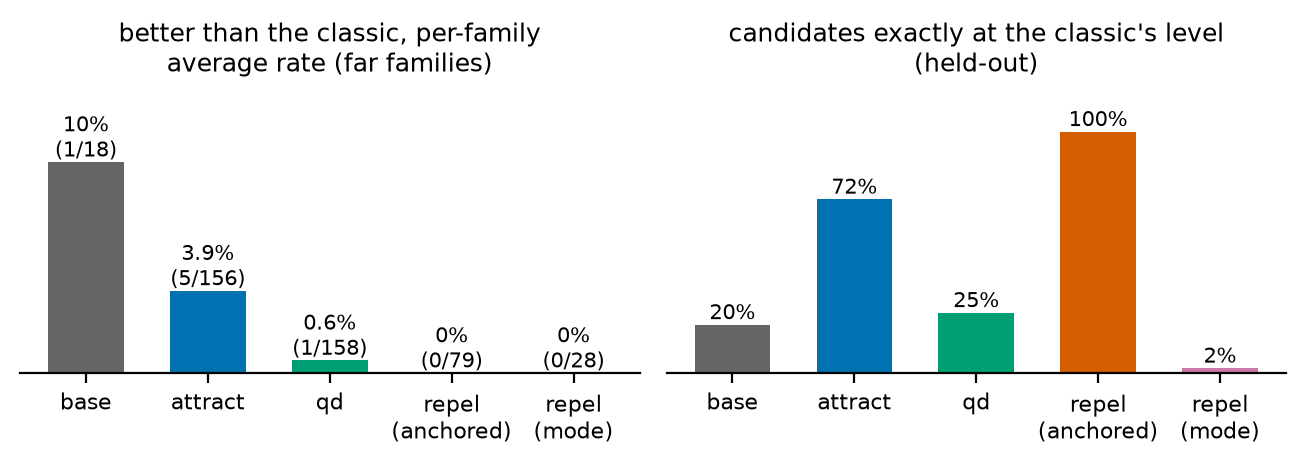
\includegraphics[width=0.9\textwidth]{fig_n_tails.png}
\caption{Consolidation pays with the tails (data from
\citet{ono2026mass}). Left: the share of candidates better than the
stronger classical heuristic on distant families, for the untrained base
(10\%), the consolidated model (\emph{attract}, 3.9\%), a
diversity-preserving objective (\emph{qd}, 0.6\%) and two repulsion
variants (0\%); bars are per-family average rates, the counts above them
pooled events (base 1/18, attraction 5/156). Right: the share of held-out
candidates exactly at the classic's level (base 20\%, attraction 72\%, qd
25\%, anchored repulsion 100\%, a functional collapse; mode repulsion 2\%).
Both panels rest on zero to five events per arm.}
\label{fig:tails}
\end{figure}

\paragraph{Consolidation moves the mass and pays with the tails.} A LoRA
trained on the model's own verified findings shifts what it writes next
toward the value region on unseen variants, by the same amount in three
lineages; the best candidate does not move (the classical heuristic, to six
decimals, in every lineage); and the share of better-than-classic
candidates in a distant family falls from 10\% to 3.9\% under attraction
and to at most 0.6\% under every other adapter (Figure~\ref{fig:tails}),
anchored repulsion delivering the entire mass to the best-known attractor.
Per notebook, attraction's larger production still yields more such
candidates (five against one); both readings rest on zero to five events
per arm \citep{ono2026mass}: the concentration is established, the cost in
discovery is per candidate and preliminary.

\begin{figure}[!htbp]
\centering
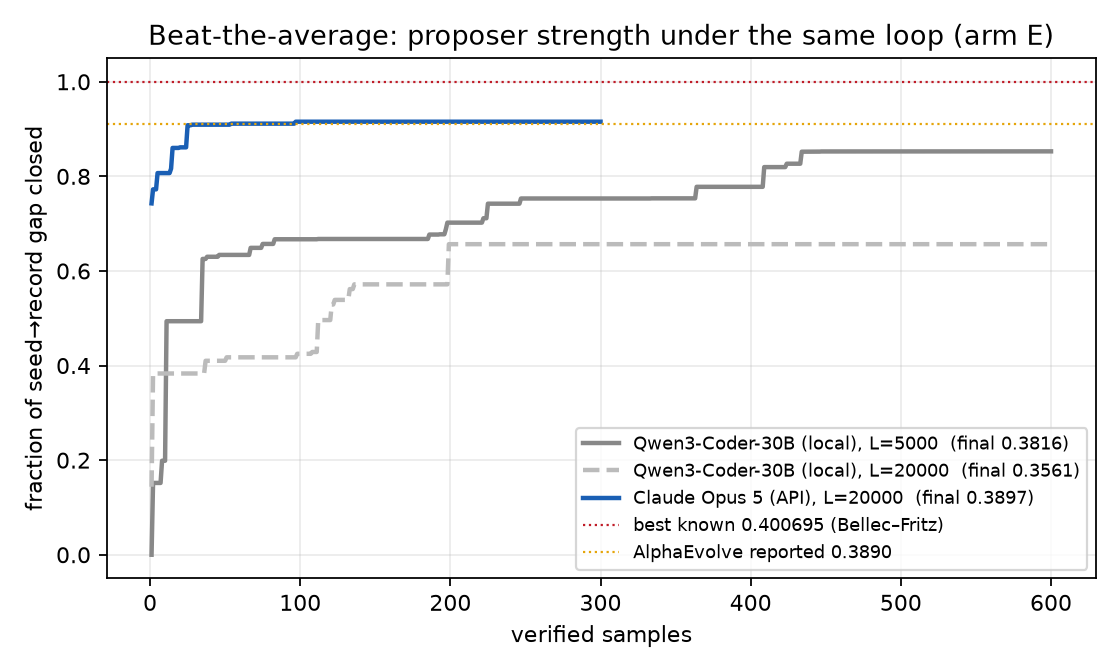
\includegraphics[width=0.78\textwidth]{fig_f4_proposer_curve.png}
\caption{The proposer curve on beat-the-average (data from
\citet{ono2026operator}): fraction of the seed-to-record gap closed against
verified samples, for the local 30B at two grid resolutions ($L=5{,}000$ and
$20{,}000$) and Claude Opus 5 at $L=20{,}000$, under the same loop. Dotted
lines mark AlphaEvolve's reported 0.3890 and the best known 0.400695
\citep{bellec2024beat}. The frontier proposer's final here is 0.3897; a
later run at the same $L$ with a tripled verifier budget reached 0.3899.}
\label{fig:wall}
\end{figure}

\paragraph{The family wall is, on the flagship problem, a resolution
limit.} Every proposer (a local 30B, a served 27B, Claude Opus 5)
stalls in the same construction family on beat-the-average, within 0.008
and a record away (Figure~\ref{fig:wall}). Five times the budget does not
move the local proposer's final and a tripled verifier time moves the
frontier proposer's by $+0.0002$; a finer grid makes the local search
harder (0.3561 at $L=20{,}000$); and the value the record's family attains
on a finite grid rises slowly with the resolution (members written for
this analysis: 0.3850 at $L=5{,}000$, 0.3867 at $20{,}000$, 0.3888 at
$4{,}000{,}000$). The record's construction is a self-similar scale
mixture whose value, 0.400695, is a continuum limit; by the argument
following their Proposition 3.3 no finitely supported distribution is
optimal, and the optimum lies between 0.400695 and 0.417
\citep{bellec2024beat}, so a family above the record is not excluded. The
600-sample finals already carry the family's structure, read by inspection
of their atoms: a dyadic ladder at the top (distances from the top
halving step by step), a smaller copy near zero, split atoms (adjacent
pairs sharing one mass) that break ties. They beat the members written
for this analysis at the same grid (0.3876 at $L=5{,}000$; 0.3899 at
$20{,}000$); the registered classifier labels only the 30B's final a
ladder, the others sparse-other (few atoms, no ladder), so this is an
inspection reading. The last mile here is the continuum limit; the family
was in the loop's hands, which is not the problem being exhausted. Family
walls on the other shared plateaus (isosceles-free subsets, $180!$) remain
hypotheses.

\section{Handing an idea}
\label{sec:handed}

If stimulation cannot produce the idea, what does the model do when the
idea is handed to it? Four experiments asked: the family-hint test of the
third paper and the three programs after it, the last arbitrating between
the explanations the others raised.

\subsection{A family named in words is adopted and loses}
\label{sec:hint}

The decisive test of the family wall \citep{ono2026operator} handed the
loop the record's family: five conditions, three seeds each, 120 samples
per run on the local 30B (August battery, means; the factorial below is a
later battery on another backend, no-hint median 0.358). Named in words
(an atom at zero holding substantial mass and atoms accumulating
geometrically toward the maximum), the family was adopted (the finals
have its signature) and lost: 0.327 against 0.352 without any hint. Handed
as crude code (three dyadic atoms, 0.273 on its own), the loop climbed
inside the family to 0.358; handed as the oracle seed (0.374), it stayed
loyal and moved by 0.001. No unaided candidate in the three runs matched
the family signature under the registered classifier; over 600 samples the
loop does reach the structure, by inspection (Section~\ref{sec:ladder}),
and what it does not reach is the continuum limit. What survives, within
the grid, is the form result: words are instruction while code is search.

\subsection{Transfer by correspondence adds nothing to the no-source control}
\label{sec:transfer}

The second program asked whether a frontier model, given the statement of a
target problem and a verified construction from a different problem, could
propose a structural correspondence and write a transplant that takes the
search loop out of the family in which it stalls. The target was
sum-difference III: best unaided final 1.112, in the family $F_0$ of sums
of a few powers of two; AlphaEvolve's published 1.148 (2{,}003 integers,
under the harness cap); best known 1.173. The library held 84 executable
constructions from nine other problems and twelve classical families, the
record's own family excluded. Two proposers ran, Claude Opus 5 and Kimi
K2.6. The pre-registered primary contrast, correspondence against a
syntactic sham that never saw the target, was formally positive for
Opus: 78 of 84 entries produced a candidate outside the stalled family,
against 1 of 84 for the sham. The no-source control, registered before it
was run, undid the reading: the target statement alone produced 73 of 84
(paired $p=0.33$) and the better best score (1.1240 against 1.1198). The
best transplants were the same program regardless of the source: the
record's mechanism, a carry-free digit encoding (digits chosen so that
sums never carry), reconstructed from the prior in 79 of 146 valid
no-source transplants. The rate of exits was uniform across source
groups: the source left no mark. Kimi produced 2 of 84 exits with a source
and 0 of 84 without. A local loop seeded with the top transplants did not
improve the strong seeds, and the no-source arm matched or exceeded the
correspondence arm (Appendix~\ref{app:stage2}). One frontier model
reconstructs the strong family from the target alone, another does not,
and a cheap loop carries neither further.

\subsection{A same-kind example buys the exit from reasoning within a small budget}
\label{sec:bridges}

The third program moved to a setting where the ``idea'' is an intermediary
with a verifier: the two Lean worlds that passed a calibration gate
(baseline 1/4, oracle 4/4; 4--5 September). A proposer session must
produce a bridge; a recipient session that never saw the proposer's work
receives it and attempts a hidden sibling. The proposer is Claude Opus 5
through Amazon Bedrock, submitting through a function call, with 16{,}384
output tokens per response, up to twelve tool turns and 600 s per session
unless stated.

At 16{,}384 tokens, production needs a trigger. Given the target alone,
the proposer reasons until the output limit and never submits (0/2, then
0/4). Given a worked example of the same kind of intermediary, relevant
or a matched sham with the wrong content, it produces a valid bridge in
one to two and a half minutes (4/4; 5{,}400--14{,}700 output tokens). The
bridges transfer: recipients solve the hidden siblings 7/8 times with a
produced bridge (the four bridges of the two example arms, each tried on
both siblings), 4/4 with the oracle, 0/4 without one in this battery (2/4
in an earlier battery at 16{,}384; 0/4 at 8{,}192). A trigger ablation
(five arms, Appendix~\ref{app:budget}) found that neither an example from
an unrelated domain, nor an instruction to submit early, nor the
\emph{kind} of intermediary in words, nor the kind in words plus an order
to write one's own example does the work (0/4 each, the last four
responses a single block of thinking at the cap); a file skeleton with no
mathematics gave 1/4. Across the ablation 23 of 24 sessions without a
same-kind example ended at the cap without a submission.

A pre-registered sensitivity then gave the two arms with nothing of the
kind in operable form, the target alone and the kind in words plus the
order to write one's own example, two and four times the cap (32{,}768
and 65{,}536 tokens per response, the session cap being the response cap
plus 16{,}384, the session time limit raised from 600 s to 3{,}600 s), two
worlds $\times$ two replicates per cell, with the reading rule fixed before
any call: any valid bridge reads the ablation's null as censored. The
transport changed during the run: the first two 32{,}768-token requests
returned nothing within the 2{,}400 s request limit through the
non-streaming path, a prospective amendment switched to a streaming client
with the same request body, and the four cells without a model verdict
were rerun once under new identifiers, as the plan provided (one of the
four reruns succeeded). Under those conditions the target alone produced a
valid bridge in 1 of 4 sessions at 32{,}768 tokens and 3 of 4 at 65{,}536,
the kind in words in 2 of 4 and 3 of 4: at 32{,}768 only in the
representation world, at 65{,}536 in both (Appendix~\ref{app:budget}). The
successes spent 14{,}000--78{,}000 output tokens over one to three responses
and 163--803 s, against 5{,}400--14{,}700 tokens and 61--161 s for the four
sessions with a same-kind example; two of the six successes at 65{,}536,
both in the invariant world, exceeded the ablation's 600 s limit, so under
that limit the 65{,}536 reading would be 2 of 4 and 2 of 4, in the
representation world only. The failures again ended at the cap; the
example arms were not rerun at the larger caps. The null of the ablation
was censored by the budget, as the recipient side had suggested. What the
same-kind example buys is the exit from reasoning within a small budget
(the bridge in a minute or two rather than in up to thirteen minutes,
or not at all at 16{,}384 tokens), not an operator the prior lacked: on
these development worlds the proposer writes the intermediary from the
target alone when given the room. Two open models placed in the same
worlds sat at a floor (Qwen3.8-27B) or, on simpler algebraic tasks of the
same construction, at a ceiling with and without a bridge (27B) or with no
contrast (Qwen3.5-4B); no target for activation patching was found
(Appendix~\ref{app:budget}).

\subsection{The factorial: form, slot, persistence}
\label{sec:factorial}

The family-hint result and the trigger series said the same thing in two
families at the budgets first tried (handed as code a family is tuned,
named in words it is obeyed and lost; a same-kind example as code triggers
production at 16{,}384 tokens where the kind in words does not), but the
original data confound three explanations: the code was always in the seed
slot and transient (a weak seed is displaced in the first generation), the
words always in the hint slot and persistent, and a re-reading of the
August runs with a frozen family detector showed the difference in
obedience this makes (79\% of valid proposals in the family under the
words hint, 10\% with the crude code as seed; Appendix~\ref{app:factorial}).
Three hypotheses were registered. \emph{Form}: code versus words, because
from a description the model writes a poor instance the loop does not
tune, while from code it makes local edits that pay. \emph{Slot}: an
object to mutate or an instruction to obey (registered prediction: seed
above hint). \emph{Persistence}: whether the content stays (registered
prediction: transient above persistent).

The battery crossed the three factors with the same content: the crude
family code or the family in words, in the hint slot or as the seed
program, persistent (hint in every generation; seed pinned as an extra
version) or transient (hint in generation 0 only; seed shown while elite);
four reference and continuation arms (no hint, the oracle code, the
model's own words-derived implementation as seed, the crude code as seed
\emph{plus} the words as hint). Twelve arms, four RNG seeds, 120 samples
per run, Qwen3-Coder-30B-A3B served in bf16, the same loop as before;
outcomes, reading rule and the gate for the mechanistic follow-up fixed
before any generation. Primary outcome: the final best; secondary: the
share of valid proposals in the family, over the run and in generation 0.
The two cells of a pair share the sampler's RNG seed, not the trajectory.

\begin{figure}[!htbp]
\centering
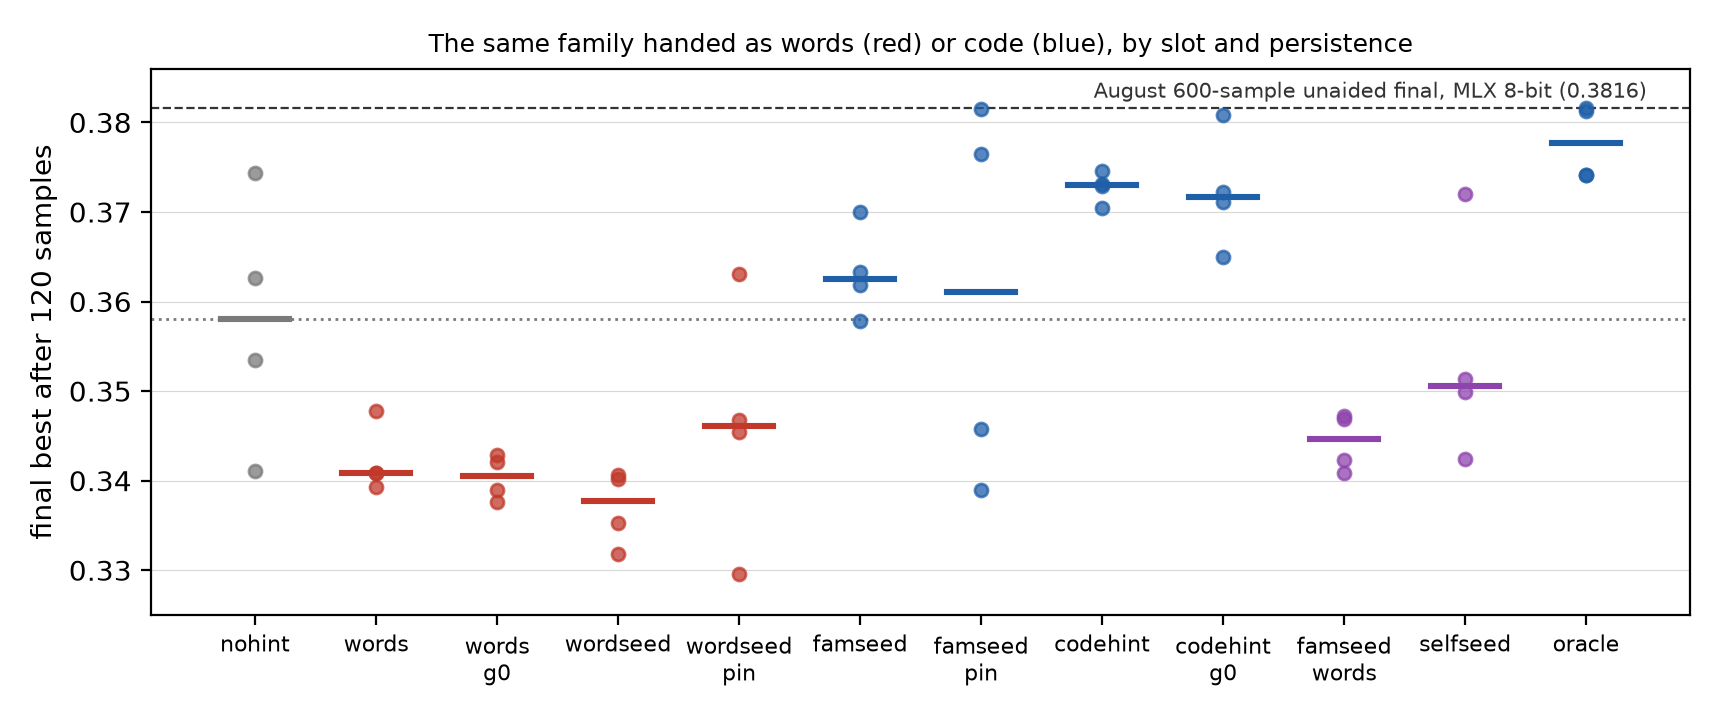
\includegraphics[width=\textwidth]{fig_slot_arms.png}
\caption{The factorial battery, final best per run (4 RNG seeds per arm;
bars are medians). Red: the family in words; blue: the family as crude code
and, at the right, as the oracle code; purple: code plus words, and the
model's own code written from the words. Dotted: the no-hint median.
Dashed: the August 600-sample unaided final of the same proposer family
(0.3816), on the MLX 8-bit backend of the earlier batteries, not the bf16
backend of this one. What to see: all four red medians sit below the dotted
no-hint line, all four blue medians above it, the purple ones between.}
\label{fig:slot}
\end{figure}

\begin{table}[!htbp]
\centering\footnotesize
\setlength{\tabcolsep}{4pt}
\begin{tabular}{l rr rr rr}
\toprule
factor (level $-$ level) & final & $+/-/0$ & family & $+/-/0$ & family g0 & $+/-/0$ \\
\midrule
form (code $-$ words) & +0.0292 & 14/2/0 & +0.21 & 15/1/0 & +0.33 & 14/1/1 \\
slot (seed $-$ hint) & -0.0027 & 6/10/0 & -0.29 & 2/14/0 & -0.17 & 2/12/2 \\
persistence (transient $-$ persistent) & -0.0026 & 6/10/0 & -0.31 & 3/13/0 & +0.00 & 7/4/5 \\
\midrule
C1: famseed\_words $-$ famseed & -0.0185 & 0/4/0 & \multicolumn{4}{l}{ranges disjoint} \\
C4: selfseed $-$ words & +0.0105 & 3/1/0 & \multicolumn{4}{l}{ranges overlap} \\
R: famseed $-$ words (replication) & +0.0217 & 4/0/0 & \multicolumn{4}{l}{ranges disjoint} \\
\bottomrule
\end{tabular}

\caption{Factorial main effects (paired differences over the four cell
pairs that differ only in the factor, four seeds each: median and sign
count $+/-/0$ of 16) on the final best, the family share over the run, and
the family share in generation 0; and the pre-registered contrasts
(per-seed differences, sign count of 4). Dominance rule, registered: the
larger paired median with at least 12 of 16 concordant signs (two-sided
binomial $p\approx0.08$ under independence; 14 of 16, $p\approx0.004$).
Per-arm finals in Appendix~\ref{app:factorial}.}
\label{tab:effects}
\end{table}

Form is dominant by the registered rule (Table~\ref{tab:effects},
Figure~\ref{fig:slot}): code beats words by 0.029 in the median, in 14 of
16 pairs and in all four cell medians (in the pinned-seed combination two
of four pairs go the other way). The four words cells sit \emph{below} no
hint (medians 0.338--0.346 against 0.358) and the four code cells above it
(0.361--0.373). Slot ($-0.003$, 6/10) and persistence ($-0.003$, 6/10)
have no main effect on the final; they move only how much the model obeys
(a persistent hint is followed in 76\% of proposals for words, 86\% for
code; shown once, in 10\% or 29\%), and following it does not help. The
registered contrasts: C1, code plus words minus code, predicted below zero
under the slot and persistence hypotheses and near zero under form, came
out at $-0.019$, 4/4, disjoint ranges: adding the correct description of
the family to a run that already has its code drops the final from 0.363
to 0.345, the level of words alone, with 86\% of proposals obeying the
description; next to the code the correct description is harmful. C4, the
model's own code written from the words and handed back as a seed, minus
words, predicted above zero under all three hypotheses, came out at
$+0.011$ with 3/1 signs and overlapping ranges, and that seed climbed by
0.022 where the trivial seed climbs by 0.087, a poor basin. R, the
August contrast, replicated ($+0.022$, 4/4, disjoint). The mechanism
offered below (obedience displaces optimisation) is the post-hoc
synthesis of these three readings, not a consequence of the form
hypothesis alone. A descriptive interaction (the same crude code does
better in the hint slot than as a seed) does not survive matching on
persistence with disjoint ranges, and the registered gate for a
mechanistic follow-up did not open (Appendix~\ref{app:factorial}).

\section{Why stimulation had a ceiling here: a conjecture}
\label{sec:why}

The seven substrates and the four delivery experiments admit one
description, stated as a conjecture with its boundary rather than as an
argument, because the quantity that would make it an argument, a bound
on the conditional mass the prior places near a target, was not
measured.

\paragraph{No inference-time stimulus raised verified value above what the
unaided or no-source condition already produced.} The sampler moved the
surface, not the ideas. Interruption bought variation because a new
subject conditions the prior on a region it already contains, and never
bought progression because nothing in the stream updates the prior; the
fabricated verdicts are the prior producing the surface of a reward it
cannot earn. The state pulse carried content the prior already reads (its
shams show that the content of the direction is what acts) and trailed the
written word at every matched offset. Consolidation, the only intervention
that changes the prior, moves the mass toward what the verifier approved
and away from the tails. The ceiling was measured with margin only on
sum-difference III, where the record's family fits under the harness cap
(1.1236 against 1.112) and 84 plus 84 entries and 108 runs never left
1.124; elsewhere the nulls sit on a floor (best fit near-optimal; no
headroom on the verified carrier of the state study), a grid limit
(beat-the-average) or a budget (the formal worlds), which makes this part
and the third less independent than they look.

\paragraph{An operator that is handed is used if it arrives in operable
form.} The search loop is a local editor of objects present in its
context: it mutates programs, keeps the ones the verifier scores higher,
and shows them again. Code is such an object; a description is not. Handed
code, the loop edits it and the family propagates through the elites.
Handed a description, the model obeys it, and the instance it writes is
poor (its own translations score 0.31--0.34 against 0.374 for the oracle
seed, and tuning them yields a quarter of what tuning the trivial seed
yields); the description then competes with the search, pulling proposals
toward its own weak instances, so a run with the code and the description
ends where a run with the description alone ends. This is why words lose
below the no-hint baseline and why the correct description hurts next to
the correct code: obedience displaces optimisation, the post-hoc
synthesis of the three registered contrasts, consistent with all three
hypotheses and predicted in full by none. The formal worlds show the same
asymmetry without a loop, at a small budget: told the kind of object to
build, the proposer reasons to the cap and submits nothing; told to write
its own example first, the same; shown an example of that kind as code,
even with the wrong content, it produces a valid bridge in minutes; given
four times the cap, it produces one without any example in three of four.
The example is not information about the target (the sham has none); it is
the operator in operable form, and what it buys is the switch from
reasoning to submitting.

\paragraph{The half that is not established: fabricating an operator the
prior lacks.} Fabrication, operationally: producing an operator that the
same proposer's no-source control does not produce at any budget at which
that control finishes without being censored by the cap. The clause
matters: at 16{,}384 tokens the example arm produced 4/4 and the no-source
control 0/4, which the definition without it would call fabrication and
which the sensitivity showed to be a budget effect. By that definition
neither delivery program observed fabrication: the transfer program's
no-source control produced the record's family as often as the
correspondence did (recall, not transfer), and the formal worlds' no-source
control produced nothing at 16{,}384 tokens and the intermediary in 3 of 4
sessions at 65{,}536. The operator was in the prior; the example bought the
exit from reasoning within a small budget. ``In the prior'' is therefore
relative to the largest budget tried, and the boundary recedes as the
budget grows, one more reason why only a blind target decides. The
sentence the program ends on: the model operates on what it receives in
operable form, and, on the targets tested, what the operable form bought
was time within a budget, never an operator the no-source control could
not produce given the room. Whether the model fabricates an operator absent
from its prior is not testable on a target with a literature, nor on
development worlds whose operators the prior evidently contains, because a
positive there is recall of low mass and fabrication alike; it is testable
on a blind target, and Section~\ref{sec:organ} says where. This is a
description of every result obtained, not a theorem; the position that
language models cannot jump \citep{zahavy2026jump} reaches a related
conclusion from the theory side and is contested, and the present series is
a measured version of one of its halves, with the currencies named and the
ceiling located within a budget.

\paragraph{What the literature already predicted.} That a sham with the
wrong content triggers production, and, after the sensitivity, that the
whole formal-world effect is one of format and latency, is what the
format account of in-context learning predicts: demonstrations act through
their format and input distribution as much as through the correctness of
their content \citep{min2022rethinking}. That code elicits what words do
not is the finding of program-aided prompting \citep{gao2023pal,chen2023pot}
and of code prompting for conditional reasoning \citep{puerto2024code};
what the factorial adds is the \emph{damage} done by a correct description
next to the code, a case of distraction by competing context
\citep{shi2023distracted} with the distractor a true statement about the
object being optimised, and that the asymmetry survives a search loop with
the same content in two forms. What the series adds to each is the
verifier: the effect is measured on verified value, paired over seeds,
with the sham and the no-source control in the design.

\section{What would not have a ceiling, and its price}
\label{sec:organ}

The one movement that shortens the distance in bits is updating the prior
on what the world approved, and the series measured its price: the tails.
The rule the program arrived at (train to exploit, propose with the raw
prior, select with the world) is one side of an open dispute in the
RL-with-verifier literature at fixed budget: sharpening raises pass@1 and
lowers pass@$k$ for large $k$, predicted by the base prior
\citep{yue2025rlvr}, the support argument has been made formally
\citep{wu2025leash}, sampling the raw model more often beats sharpening it
\citep{brown2024monkeys}, and diversity-preserving objectives are an active
repair \citep{li2025darling,zhang2025verbalized}; on the other side,
prolonged reinforcement learning reports pass@$k$ above the base even where
the base fails at every $k$ \citep{liu2025prorl}.

Where consolidation did produce discovery beyond what the base samples in a
finite budget is the one place this program did not go: updating the
weights \emph{on the problem itself}, at test time, with width. ThetaEvolve
runs reinforcement learning on a single open problem with an 8B open model
and a bank of ten thousand programs, and passes AlphaEvolve's
circle-packing value (2.63598 against 2.63586) after 65 steps of
$32\times16$ programs, about 33{,}000, on eight A100s
\citep{wang2025thetaevolve}; TTT-Discover reports new bounds with the same
recipe, mostly on gpt-oss-120b, against a best-of-25{,}600 raw-model
baseline that lands within $3\times10^{-5}$ of it on the Erd\H{o}s
minimum-overlap problem and far behind on the engineering problems
\citep{yuksekgonul2026ttt}. In bits of budget ($\log_2$ of the verified
samples, what was spent, not the distance of Section~\ref{sec:question})
these systems spend about fifteen where this program spent seven to nine,
and they spend them by changing the prior between samples. Two facts frame
what they show: the records they move sit in the fourth or fifth decimal
of the same families (on beat-the-average no language-model system has, to
our knowledge, reported more than about 0.390, AlphaEvolve's 0.3890
\citep{georgiev2025exploration} and this program's 0.3899
\citep{ono2026operator}, against the continuum value 0.4007), and
whether an evolutionary search escapes a family at all depends on which
family it locks into first \citep[Appendix D.2, greedy
allocator]{xing2026base}.

This locates the next lever and where to test it. Every inference-time
stimulus failed to make the model produce, within the budgets tested, an
operator its no-source control does not produce; the question left is
whether weights updated on the problem, with width, can. Beat-the-average
is the wrong problem for that test: its verifier scores a grid, the grid
caps the families the loop reaches near 0.385--0.390 at the grids used, and
the loop already produces the record's family. The test needs a problem
where the record's family is representable on the verifier's grid and
beats the family the model defaults to. The transfer program named one:
sum-difference III, where the record's family scores 1.1236 within the
harness cap against 1.112 for the best unaided loop final, and the
published 1.148 lies above both. The caveat is
Section~\ref{sec:transfer}: Claude Opus 5 reconstructs that family from the
statement alone (1.1240), Kimi K2.6 does not (0 of 84). The test is
legible with a proposer whose no-source control is null at a budget at
which it is not censored (the local 30B, whose 20 unaided runs all
stayed in $F_0$, or Kimi), and decisive only on a blind target without a
literature, where recall and fabrication cannot be confused: the blind
target is the condition, not an alternative. If a test-time-learning run
there produces the record's family without being handed it, fabrication is
possible, at the price of bits and of weights that forget; if it tunes
inside the default family, the sentence extends from inference to training,
and the wall is the prior's, not the loop's. Either answer is informative,
and neither is another prompt.

\section{Practical rules and falsifiers}
\label{sec:rules}

For a verified search with a language model at office scale, the factorial
supports three rules on the tested problem and proposer family (elsewhere
they are hypotheses) and one hypothesis.
\begin{enumerate}
\item Hand ideas as code, not as descriptions. A description of the
family costs a run 0.012--0.020 against no hint; the same family as a crude
program gains 0.003--0.015, and as a good program reaches this proposer's
120-sample ceiling on this grid (0.374--0.378; the family's own grid values
are higher, Section~\ref{sec:ladder}).
\item Do not add the description to the code: the correct description next
to the correct code drops the run to the level of the description alone.
\item Spend the search budget on breadth and selection, not on stimulus
engineering: in these runs variation was cheap and never the bottleneck,
and the funnel stalled at the proposer's plateau, which no stimulus
crossed. The budget per session is a separate axis:
Section~\ref{sec:bridges} shows it turning a null into three of four.
\end{enumerate}
The hypothesis: put the code in the hint slot, framed as a known
construction. The persistence-matched comparisons
(Appendix~\ref{app:factorial}) favour it in 6 of 8 seeds with overlapping
ranges, the registered slot effect is null, and the registered slot
hypothesis predicted the opposite.

The falsifiers are specific; one was met by the sensitivity run after the
ablation. Not observed: an inference-time stimulus that raises verified
value beyond the proposer's family, on a problem whose verifier can express
the exit (beat-the-average cannot); a consolidation that raises the
better-than-classic rate in a distant family; a state channel that beats
the written word at matched offsets; a proposer that produces the record's
family without a seed of code on a blind target, or on a published target
with a proposer whose no-source control is null at an uncensored budget; a
description that a search loop tunes to the level of the operator's code,
at the 120 samples tried; a bridge from the kind in words at 16{,}384
tokens; and, for the sentence as it now reads, an example arm that
produces, on a blind target and at a budget at which the target alone
finishes uncensored, a bridge the target alone does not. Observed: a
bridge from the target alone, or from the kind in words, above 16{,}384
tokens (Section~\ref{sec:bridges}), which is why the sentence reads
``not an operator the prior lacked'' rather than ``does not fabricate the
operator'', and why fabrication is left to a blind target.

\section{Availability}
\label{sec:availability}

Papers 1--4 are public with instruments and data: arXiv:2608.19893 and
arXiv:2608.28886 (mirrored on Zenodo as 10.5281/zenodo.22714130 and
10.5281/zenodo.22714136); Zenodo 10.5281/zenodo.22280391 (version 3) and
10.5281/zenodo.22280784 (version 3, DOI of the version
10.5281/zenodo.22714155; version 2, 10.5281/zenodo.22713526, has the same
content with em-dashes); run data in the releases \texttt{run-data-v1}
and \texttt{run-data-v2} of
\url{https://github.com/RobertoOno/interrupting-the-loop}, archived as
Zenodo 10.5281/zenodo.22714138. The evidence
of programs 5--7 (per program the single-read appendix, the raw session
traces and verifier reports, the frozen analysis scripts, the transfer
library, the two Lean worlds with their verifier, and the dated
pre-registration entries of the project notebook) is deposited as Zenodo
record 10.5281/zenodo.22713807.

\section{Limitations}
\label{sec:limits}

One laboratory, one discipline, office-scale models (8B to 30B locally, a
served 27B, Claude Opus 5 through an API, Kimi K2.6 in the transfer program
and as the second judge family), nine construction problems, one
bin-packing family, two Lean world families, one primary judge family for
the text studies (a second judge family and human readers reproduced the
ordering in the first paper). The factorial has four seeds per cell and is
read as a design, not as a test with power; its dominance rule is lenient
and its interaction is descriptive. The distance in bits is quantified only
where Section~\ref{sec:organ} counts samples, as a budget; the
bits-to-threshold measure the transfer program defined was censored in
every run. The formal-world results rest on two exposed worlds and two
replicates per arm; the open-model results on one 27B and one 4B at a
floor or a ceiling. The production null of the ablation is a budget
effect, so the fabrication question stays open; the blind targets that
would test it were designed and not run. The unifying sentence is a
description of every result obtained, not a theorem, and
Section~\ref{sec:rules} says what would break it.

\bibliographystyle{plainnat}
\bibliography{references}

\appendix

\section{Objects and models}
\label{app:objects}

\begin{table}[!htbp]
\centering\footnotesize
\setlength{\tabcolsep}{3pt}
\begin{tabular}{R{2.3cm} R{6.0cm} R{6.6cm}}
\toprule
object (where) & what is produced, and how it is verified & reference values \\
\midrule
text studies (papers 1, 2, 4) & a base model continues a premise; interventions act on the sampler, the context, the weights or the residual stream; a judge scores windows of generated-only text for surprise, connection and coherence, never seeing the intervention & unit of inference: the premise (10 or 30); paired sign-flip and permutation tests; a second judge family and human readers reproduced the ordering in paper 1 \\
online bin packing (papers 1--2) & the FunSearch form: the model writes \texttt{priority(item, remaining)} heuristics; the verifier packs instances and reports the mean excess over the lower bound & best fit, the classical heuristic, is near-optimal on the ten distribution variants of the text studies and measurably beatable on the small-item family of the consolidation battery, where the best candidate of every lineage nonetheless equals it (0.021028) \\
beat-the-average (paper 3; program 7; the wall analysis in program 5) & a probability mass function on a grid of $L$ points in $[0,1]$; maximise $P[X_1{+}X_2{+}X_3<2X_4]$ for i.i.d.\ draws, computed exactly by convolution; $L=5{,}000$ unless stated & trivial seed 0.2708; unaided finals 0.3816 (local 30B, 600 samples), 0.3876 (27B, $L=5{,}000$), 0.3897 (Claude Opus 5, $L=20{,}000$; 0.3899 with a tripled verifier budget); AlphaEvolve's reported 0.3890 at $L=20{,}000$ \citep{georgiev2025exploration}; best known 0.400695, the continuum limit of a self-similar scale mixture, the optimum being bounded between 0.400695 and 0.417 \citep{bellec2024beat} \\
sum-difference III (program 5) & a set $U\ni 0$ of at most 4{,}000 non-negative integers (the harness cap); $\theta=\log(|U{-}U|/|U{+}U|)/\log(2\max U+1)+1$, exact & unaided 1.1123 (20 runs, all in $F_0$, the family of sums of at most three powers of two); the record's family, a carry-free digit encoding, scores 1.1236 within the cap when instantiated by hand; AlphaEvolve's published 1.1479 with 2{,}003 integers; best known 1.1731, with far larger sets \\
Lean worlds (program 6) & two small formal worlds in Lean 4 (an invariant preserved by every step; a change of representation with an action and an inverse), each with a visible target theorem, two hidden sibling theorems and an oracle bridge lemma that makes the siblings short; the verifier compiles the submission and checks its axioms & outcomes are counts: valid bridges (proposers) and solved siblings (recipients); two worlds $\times$ two replicates per arm \\
nine construction problems (paper 3) & circle packing, ring loading, beat-the-average, the first autocorrelation inequality, isosceles-free subsets, sum-difference III, max--min distance, the Heilbronn triangle, $180!$ into 180 factors, from the AlphaEvolve repository \citep{georgiev2025exploration} & outcome: the fraction of the seed-to-record gap closed; two shared plateaus (isosceles-free, $180!$) where every arm meets the same value \\
\bottomrule
\end{tabular}
\caption{The objects of the paper.}
\label{tab:problems}
\end{table}

\begin{table}[!htbp]
\centering\footnotesize
\setlength{\tabcolsep}{3pt}
\begin{tabular}{R{2.6cm} R{4.6cm} R{4.6cm} R{3.0cm}}
\toprule
role & model & precision, serving & where \\
\midrule
text generators & Qwen3-30B-A3B-Base, Qwen3-8B-Base, OLMo-2-13B & 8-bit, MLX, one laptop & papers 1--2 \\
consolidation & Qwen3-8B-Base, QLoRA & 8-bit, MLX & paper 2 \\
state-space injection & Qwen3-8B-Base (replication at 14B) & 8-bit MLX and bf16 PyTorch & paper 4 \\
judge & Claude Opus 5; second family Kimi K2.6; human readers & API (Bedrock; OpenRouter) & papers 1, 2, 4 \\
search proposer & Qwen3-Coder-30B-A3B-Instruct & 8-bit MLX (paper 3); bf16 vLLM on an H100 (program 7) & paper 3, program 7 \\
search proposer & Qwen3.8-27B & served in non-reasoning mode with a 3{,}000-token budget & paper 3 \\
search proposer & Claude Opus 5 & API & paper 3 \\
transfer proposers & Claude Opus 5; Kimi K2.6 & Bedrock; OpenRouter & program 5 \\
stage-2 loop & Qwen3-30B-A3B-Base & vLLM completions on an H100 & program 5 \\
bridge proposer and recipients & Claude Opus 5 & Bedrock; submission through a function call; 16{,}384 output tokens per response (32{,}768 and 65{,}536 in the budget sensitivity) & program 6 \\
open-model contrast & Qwen3.8-27B; Qwen3.5-4B & vLLM on an H100, files in fenced code blocks, no tool; FP32 on an RTX 4090, submission through a function call & program 6 \\
\bottomrule
\end{tabular}
\caption{The models, by role.}
\label{tab:models}
\end{table}

\section{The factorial in detail}
\label{app:factorial}

\paragraph{The August runs re-read.} Before any new data, the exposed
August runs of the family-hint test were re-read with the frozen family
detector (a geometric ladder of atoms toward the top with an atom at zero;
at least three steps, consecutive ratios in $[0.2, 0.95]$, coefficient of
variation at most 0.35, first step at least 100 positions below the top).
Under the words hint 79\% of all valid proposals were in the family, with
the crude code as seed 10\% (the seed having been displaced at once), with
the best hand-written seed 72\%, because it stayed elite by merit.

\begin{table}[!htbp]
\centering\footnotesize
\setlength{\tabcolsep}{2.5pt}
\begin{tabular}{llll rrrr}
\toprule
arm & content & slot & persistence & median & range & family & family g0 \\
\midrule
nohint & --- & --- & --- & 0.3581 & 0.3411--0.3744 & 0.09 & 0.00 \\
words & words & hint & persistent & 0.3408 & 0.3393--0.3478 & 0.76 & 0.14 \\
words\_g0 & words & hint & gen.\ 0 only & 0.3405 & 0.3377--0.3429 & 0.10 & 0.30 \\
wordseed & words & seed & transient & 0.3377 & 0.3319--0.3407 & 0.02 & 0.00 \\
wordseed\_pin & words & seed & pinned & 0.3461 & 0.3295--0.3630 & 0.07 & 0.00 \\
famseed & crude code & seed & transient & 0.3626 & 0.3579--0.3700 & 0.27 & 0.39 \\
famseed\_pin & crude code & seed & pinned & 0.3611 & 0.3389--0.3815 & 0.29 & 0.29 \\
codehint & crude code & hint & persistent & 0.3731 & 0.3704--0.3746 & 0.86 & 0.48 \\
codehint\_g0 & crude code & hint & gen.\ 0 only & 0.3717 & 0.3650--0.3808 & 0.29 & 0.54 \\
famseed\_words & crude code + words & seed + hint & persistent & 0.3446 & 0.3409--0.3473 & 0.86 & 0.80 \\
selfseed & own code from the words & seed & by merit & 0.3506 & 0.3424--0.3720 & 0.17 & 0.33 \\
oracle & best hand code & seed & by merit & 0.3777 & 0.3742--0.3816 & 0.39 & 0.31 \\
\bottomrule
\end{tabular}

\caption{Final best per arm (median and range over four seeds) and the
share of valid proposals in the family, over the run and in generation 0.}
\label{tab:arms}
\end{table}

\paragraph{The descriptive interaction, not registered.} The same crude
instance reaches 0.373 when handed in the hint slot (``one known family of
strong constructions, as a program'') and 0.363 when handed as the seed
program (Table~\ref{tab:arms}). That comparison crosses two factors, since
the hint is persistent and the seed transient. Matched on persistence the
picture is weaker: persistent hint against pinned seed, seeds 11--14,
$-0.008$, $+0.025$, $-0.002$, $+0.034$, 2 of 4 with overlapping ranges;
generation-0 hint against transient seed, $+0.014$, $+0.001$, $+0.003$,
$+0.018$, 4 of 4 with overlapping ranges (0.365--0.381 against
0.358--0.370). In the seed slot the instance appears as ``Version 0, score
0.2734'' and is often abandoned (27\% adoption, two of four finals in the
family); in the hint slot it is adopted by half of the first generation
and tuned, with all four finals in the family, even when the hint is shown
once. That the slot carries credibility (the seed block displays the
weak score, the hint block lends authority) is a hypothesis for a test
of its own, at $n=4$; the registered slot effect is null and the registered
slot hypothesis had predicted the opposite direction.

\paragraph{The gate.} The gate for the mechanistic follow-up required a
slot effect visible in generation 0 with the same sign in both contrasts,
a design choice: activation patching in a single forward pass with
identical tokens is the cleanest contrast, not the only one
\citep{zhang2024patching}. The two generation-0 contrasts have opposite
signs and overlapping ranges. The gate did not open.

\section{The second stage of the transfer program}
\label{app:stage2}

The top transplants of each arm seeded a local loop (Qwen3-30B-A3B-Base
through a completions interface, 22--60\% valid proposals, its bare loop
below its August level; 108 runs of 200 proposals). The loop did not
improve the strong seeds: in the no-source arm the mean best rose from
1.1192 to 1.1197 over 15 runs, no run of the 108 reached half the gap to
1.148, and with the seed as the unit the no-source arm matched or exceeded
the correspondence arm ($p=0.056$--$0.063$, no-source $\ge$
correspondence). The bits-to-threshold measure defined for this stage
($\log_2$ of the index of the first valid sample closing half, or nine
tenths, of the seed-to-record gap) was censored in every run.

\section{The formal worlds: budget sensitivity and open models}
\label{app:budget}

\paragraph{The proposer budget sensitivity.} Pre-registered on 11
September 2026 before any call, with the reading rule fixed (any valid
bridge in the target-alone or kind-in-words arm at 32{,}768 or 65{,}536
tokens reads the ablation's null as censored). Same two worlds, prompts,
contract and verifier as the ablation; caps per response 32{,}768 and
65{,}536, session cap the response cap plus 16{,}384, session time
3{,}600 s, request time 2{,}400 s, twelve turns. The first two
32{,}768-token requests returned nothing within 2{,}400 s through the
non-streaming path; a prospective amendment switched the transport to a
streaming client with the same request body, and the four cells without a
model verdict were rerun once under new identifiers, as the plan provided.
Sixteen sessions, US\$19.88 at list rates.

\begin{table}[!htbp]
\centering\footnotesize
\setlength{\tabcolsep}{3pt}
\begin{tabular}{R{2.3cm} R{1.1cm} R{2.0cm} R{1.1cm} R{2.9cm} R{2.0cm} R{2.6cm}}
\toprule
arm & cap & world & bridges & output tokens of the successes (responses) & time of the successes (s) & failures: time at the cap (s) \\
\midrule
target alone & 32{,}768 & invariant & 0/2 & & & 357; 370 \\
target alone & 32{,}768 & representation & 1/2 & 22{,}175 (1) & 239 & 363 \\
target alone & 65{,}536 & invariant & 1/2 & 69{,}621 (2) & 730 & 692 \\
target alone & 65{,}536 & representation & 2/2 & 48{,}048 (2); 50{,}940 (1) & 535; 578 & \\
kind in words & 32{,}768 & invariant & 0/2 & & & 359; 373 \\
kind in words & 32{,}768 & representation & 2/2 & 22{,}365 (2); 14{,}079 (1) & 247; 163 & \\
kind in words & 65{,}536 & invariant & 1/2 & 77{,}940 (3) & 803 & 706 \\
kind in words & 65{,}536 & representation & 2/2 & 21{,}783 (1); 42{,}964 (1) & 243; 466 & \\
\bottomrule
\end{tabular}
\caption{The proposer budget sensitivity, per cell. Reference at 16{,}384
tokens (the ablation): target alone 0/4, kind in words 0/4, every session
at the cap. The four sessions with a same-kind example at 16{,}384 (the
production diagnostic) spent 5{,}358--14{,}666 output tokens and 61--161 s.}
\label{tab:budget}
\end{table}

\paragraph{The trigger ablation.} Five arms, two worlds $\times$ two
replicates, all at 16{,}384 output tokens, read once: a worked example from
an unrelated domain (arithmetic induction) 0/4; the two output files as a
skeleton with no mathematics 1/4; an instruction to submit a candidate
early and revise 0/4; the \emph{kind} of intermediary in words (``look for
a quantity every step preserves'') 0/4; the kind in words plus an order to
first write one's own worked example of that kind on a toy system 0/4, all
four responses a single block of thinking at the cap. Reference: the
target alone 0/2 then 0/4; a same-kind example, relevant or sham, 4/4.

\paragraph{The open models.} Two open models were placed in the same
worlds to look for a behavioural contrast for interpretability work.
Qwen3.8-27B, writing its files inside fenced code blocks with no tool (up
to six turns, 900 s per session): 2 of the 45 recipient cells run solved a
sibling, both with the oracle bridge at 16{,}384 tokens with thinking on,
and 1 of the 23 proposer cells run produced a valid bridge (four cells were
lost to a launcher defect): a floor, not a contrast. In simpler
algebraic tasks of the same construction (paths and invariants in a finite
matrix family) the same 27B sat at the ceiling with and without a bridge
(12/12, 8/8 and 9/12 across three batteries, the third's three failures
being time limits on the mixed path with and without a bridge), and a 4B
model (Qwen3.5-4B) on those tasks solved 6/12 without a bridge, 7/12 with
the oracle bridge and 5/12 with a sham, its delivery controls 4/4. Where
the open models solve, they solve as well without the bridge; where they
fail, in the Lean worlds, the two successes were with it. No target for
activation patching was found, and the mechanistic branch was archived
with that reading.

\end{document}
